\documentclass{article}
\usepackage{unipr_org_notes}
% grafici
\usepackage{pgfplots}
\usepackage{float}
\usepackage{tikz}
\usepackage{verbatim}
\usetikzlibrary{positioning}


\renewcommand{\coursetitle}{Analisi statica e verifica del software}
\renewcommand{\arraystretch}{1.3} % spaziatura uniforme nelle tabelle

% \addauthor{Nome}{Mail}


\renewcommand{\authorname}{Simone Colli, Manuel Di Agostino}
\renewcommand{\authoremail}{simone.colli@studenti.unipr.it, manuel.diagostino@studenti.unipr.it}

\renewcommand{\notedate}{%
    Appunti del corso tenuto dal \textbf{Prof. Vincenzo Arceri} \\
    \medskip % Aggiunge un piccolo spazio verticale
    Università degli Studi di Parma \\
    Anno Accademico 2025/2026
}


\begin{document}
\maketitle

\tableofcontents

\section*{Disclaimer}

\vfill
\begin{nota*}{}
I seguenti appunti sono stati generati a partire dal materiale
didattico e dalle note ufficiali del corso 'Analisi statica e verifica del software'.
Il contenuto è stato riorganizzato, formattato e parzialmente rielaborato con
l'ausilio di AI al fine di creare un documento coeso e ottimizzato per lo studio.

\medskip

Si raccomanda di fare sempre riferimento al materiale originale fornito dal
docente per garantire la massima accuratezza.
\end{nota*}
\vfill

\section{Introduzione}

\subsection{Cos'é l'affidabilità del software?}

\begin{definizione}{Affidabilità del Software (IEEE 610.12\-1990)}{ieee610121990}
"The ability of a system or component to perform its required functions
under stated conditions for a specified period of time"

Ovvero:

"La capacità di un sistema o componente di eseguire le funzioni richieste
in condizioni specificate per un periodo di tempo specificato"
\end{definizione}

\begin{definizione}{Gestione dell'Affidabilità del Software (IEEE 982.1\-1988)}{ieee98211888}
"The process of optimizing the reliability of software through a program that
emphasizes software error prevention, fault detection and removal, and the
use of measurements to maximize reliability in light of project constraints
such as resources, schedule and performance"

Ovvero:

"Il processo di ottimizzazione dell'affidabilità del software attraverso un
programma che enfatizza la prevenzione degli errori software, il rilevamento
e la rimozione dei guasti, e l'uso di misurazioni per massimizzare l'affidabilità
alla luce dei vincoli del progetto come risorse, tempi e prestazioni"

\end{definizione}

Sfruttando le definizioni \ref{def:ieee610121990} e \ref{def:ieee98211888},
è possibile riassumere che l'affidabilità del software consiste in 3 attività:
\begin{itemize}
    \item Prevenzione degli errori.
    \item Rilevamento e rimozione dei guasti.
    \item Valutazione per massimizzare l'affidabilità, in particolare valutazioni
    a supporto delle prime due attività.
\end{itemize}

\subsection{Perché l'affidabilità del software è importante?}

L'importanza dell'affidabilità del software deriva dalle enormi conseguenze
economiche e operative che i bug possono causare.

Alcune stime indicano che:
\begin{itemize}
    \item I bug nei software costano circa \(60\) miliardi di dollari all'anno
    negli Stati Uniti.
    \item L'economia mondiale perde circa \(250\) miliardi di dollari all'anno
    a causa di qualsiasi tipo di attacco palese (overt attack).
    \item I difetti nel software rendono la programmazione molto dolorosa.
\end{itemize}

Alcuni esempi di fallimenti dovuti a bug software includono:
\begin{itemize}
    \item Il disastro del volo 501 di Ariane 5 nel 1996, che è esploso dopo 37 secondi
    dal decollo a causa di un errore di overflow durante la conversione da un float 64 bit ad un intero 16 bit.
    Questo evento ha causato una perdita di circa \(370.000.000\) dollari.
    \item Il bug del Pentium FDIV nel 1994, che ha causato errori di calcolo
    nelle divisioni in virgola mobile. Questo bug ha portato a una perdita di
    circa \(475.000.000\) dollari.
    \item L'aggiornamento difettoso di CrowdStrike nel 2024, che ha causato
    più di \(5000\) voli cancellati. Questo evento ha impattato su banche,
    governi e infrastrutture critiche. Le perdite economiche sono state
    stimate a circa \(5.400.000.000\) dollari.
\end{itemize}

La lista di esempi potrebbe continuare, ma l'importante è comprendere
che l'affidabilità del software è cruciale per evitare perdite economiche
significative e garantire il corretto funzionamento dei sistemi.

\subsection{Validazione e Verifica}

La validazione e la verifica sono due processi distinti ma complementari
nell'ambito dello sviluppo del software, entrambi mirati a garantire che
il software soddisfi i requisiti e funzioni correttamente.


La \textbf{validazione} si concentra sulla domanda: "Stiamo costruendo il
prodotto giusto?".
Essa verifica che il software soddisfi le esigenze e le aspettative degli
utenti finali.
La \textbf{verifica}, d'altra parte, si concentra sulla domanda: "Stiamo
costruendo il prodotto nel modo giusto?".
Essa assicura che il software sia sviluppato correttamente secondo le
specifiche tecniche e i requisiti di progetto.


\begin{figure}[H]
    \centering
    
\includegraphics[width=0.8\textwidth]{images/th_01/01.png}
    \caption{L'immagine illustra la differenza tra validazione e verifica.}
    \label{fig:th_01_01}
\end{figure}

\begin{esempio}{Risposta dell'ascensore}{elevator_response}

Un esempio pratico di validazione e verifica può essere trovato nel
comportamento di un sistema di risposta dell'ascensore.

Una specifica validabile ma non verificabile potrebbe essere:
"Se un utente preme il pulsante di richiesta a un piano $i$, un ascensore
disponibile deve arrivare al piano $i$ entro un tempo ragionevole".

Una specifica verificabile è:
"Se un utente preme il pulsante di richiesta a un piano $i$, un ascensore
disponibile deve arrivare al piano $i$ entro 30 minuti".

\end{esempio}

\subsection{Verifica del Software}

Lo scopo della verifica del software è verificare alcune affermazioni di
correttezza riguardante un programma:
\begin{itemize}
    \item La \textbf{correttezza funzionale}, ovvero che il programma
    soddisfi i requisiti funzionali specificati.
    \item L'\textbf{assenza di errori non funzionali} (non cosa fa il
    programma, ma come lo fa), come ad esempio: soddisfacimento di vincoli
    spaziali e/o temporali, assenza di errori a runtime, soddisfacimento di
    vincoli di sicurezza, ecc.
\end{itemize}

\section*{Bad news: there’s no silver bullet}

Non esiste un metodo di verifica che sia contemporaneamente:
\begin{itemize}
    \item \textbf{Automatico}: non richiede interazione umana.
    \item \textbf{Potente}: è in grado di dimostrare proprietà non banali (\emph{non-trivial properties}).
    \item \textbf{Corretto (Sound)}: non dimostra mai una proprietà se questa non è vera.
    \item \textbf{Completo (Complete)}: dimostra sempre la proprietà se essa è vera e non fallisce mai nel dichiarare la correttezza di un programma corretto.
\end{itemize}

Il \textbf{teorema di Rice} afferma che tutte le proprietà non banali del
comportamento di un programma scritto in un linguaggio di programmazione
Turing-completo sono indecidibili.
L'\textbf{indecidibilità} di una proprietà implica che non esiste alcun metodo
di verifica automatico che sia allo stesso tempo \textbf{corretto} e
\textbf{completo}.
\section{Background matematico}
Per poter discutere in modo rigoroso di tecniche di verifica del software,
è necessario introdurre alcuni concetti matematici di base relativi alla
teoria della computazione e alla logica formale.

\subsection{Set notation}
\begin{definizione}{Insieme}{def:set}
Un insieme (set) è una collezione di oggetti ben definiti e distinti.
La collezione stessa è considerata un oggetto a sé stante.

Dato un insieme $S$ è possibile dire che:
\begin{itemize}
    \item $s \in S$ significa che l'elemento $s$ appartiene all'insieme $S$.
    \item $S_{1}\subseteq S_{2}\triangleq\forall s\in S_{1}\Rightarrow s\in S_{2}$
    significa che l'insieme $S_{1}$ è un sottoinsieme di $S_{2}$ se ogni
    elemento di $S_{1}$ appartiene anche a $S_{2}$.
    \item $S_{1}\cup S_{2}=\{s|s\in S_{1}\vee s\in S_{2}\}$ è l'unione di
    due insiemi, ovvero l'insieme di tutti gli elementi che appartengono
    ad almeno uno dei due insiemi.
    \item $S_{1}\cap S_{2}=\{s|s\in S_{1}\wedge s\in S_{2}\}$ è l'intersezione
    di due insiemi, ovvero l'insieme di tutti gli elementi che appartengono
    ad entrambi gli insiemi.
\end{itemize}
\end{definizione}


\subsection{Partial order}

\begin{definizione}{Ordine parziale}{def:partial_order}

Un ordine parziale (partial order) è una relazione binaria $\sqsubseteq$ su un
insieme $X$ che soddisfa le seguenti proprietà:

\begin{itemize}
    \item Riflessività: $\forall x \in X \Rightarrow x \sqsubseteq x$, indica che ogni elemento è
    in relazione con se stesso.
    \item Anti-simmetria: $\forall x, y \in X, (x \sqsubseteq y \wedge y \sqsubseteq x)
    \Rightarrow x = y$, indica che se un elemento $x$ è in relazione con un altro
    elemento $y$ e viceversa, allora $x$ e $y$ sono lo stesso elemento.
    \item Transitività: $\forall x, y, z \in X, (x \sqsubseteq y \wedge y \sqsubseteq z)
    \Rightarrow x \sqsubseteq z$, indica che se un elemento $x$ è in relazione con un
    elemento $y$, e $y$ è in relazione con un elemento $z$, allora $x$ è in relazione
    con $z$.
\end{itemize}

\end{definizione}

\begin{esempio}{Esempio informale di ordine parziale su $\mathbb{Z}$}{es:informal_partial_order_z}

Informalmente è possibile considerare l'insieme dei numeri interi
$\mathbb{Z}$ con la relazione "minore o uguale di" ($\leq$) come un esempio di
ordine parziale. In questo caso è possibile verificare che:

\begin{itemize}
    \item Riflessività: Per ogni numero intero $i$, vale che $i \leq i$.
    \item Anti-simmetria: Se $i_1 \leq i_2$ e $i_2 \leq i_1$, allora $i_1 = i_2$.
    \item Transitività: Se $i_1 \leq i_2$ e $i_2 \leq i_3$, allora $i_1 \leq i_3$.
\end{itemize}

\end{esempio}

\subsection{Powerset}

\begin{definizione}{Insieme delle parti}{def:powerset}

Dato un insieme $S$, definito in \Cref{def:set}, l'insieme delle parti
(powerset) di $S$ è l'insieme di tutti i sottoinsiemi di $S$, ed è indicato
con $\mathcal{P}(S)$.

Dato un insieme $S$ con $|S| = n$ elementi è possibile determinare che l'insieme
delle parti di $S$ ha $|\mathcal{P}(S)| = 2^n$ elementi.

\end{definizione}

\begin{esempio}{Alcuni esempi di powerset}{es:powerset_examples}

    Dato l'insieme vuoto $\emptyset$, il suo powerset è:
    \[\mathcal{P}(\emptyset) = \{\emptyset\}\]
    ed ha $2^0 = 1$ elemento.

    Dato un insieme $X = \{a, b\}$, il suo powerset è:
    \[\mathcal{P}(X) = \{\emptyset, \{a\}, \{b\}, \{a, b\}\}\]
    ed ha $2^2 = 4$ elementi.

    Dato l'insieme $\mathbb{Z}$ dei numeri interi, il suo powerset è:
    \[\mathcal{P}(\mathbb{Z}) = \{\emptyset, \{\ldots, -2, -1, 0, 1, 2,
    \ldots\}, \{0\}, \{1, 2, 3\}, \ldots\}\]
    ed ha un numero infinito di elementi.

\end{esempio}

Dato un powerset è possibile definire un ordine parziale $\subseteq$ su di
esso e verificare che esso soddisfa le proprietà di un ordine parziale:

\begin{itemize}
    \item \textbf{Riflessività:} $\forall X_{1}\in \mathcal{P}(X). X_{1}\subseteq X_{1}$
    \item \textbf{Anti-simmetria:} $\forall X_{1},X_{2}\in\mathcal{P}(X).X_{1}\subseteq X_{2}\wedge X_{2}\subseteq X_{1}\Rightarrow X_{1}=X_{2}$
    \item \textbf{Transitività:} $\forall X_{1},X_{2},X_{3}\in\mathcal{P}(X).X_{1}\subseteq X_{2}\wedge X_{2}\subseteq X_{3}\Rightarrow X_{1}\subseteq X_{3}$
\end{itemize}


\begin{esercizio}{Inclusione inversa su powerset}{es:inverse_powerset_order}

L'inclusione inversa su un powerset $\mathcal{P}(X)$ è un ordine parziale?
Per verificare se $\supseteq$ è un ordine parziale su $\mathcal{P}(X)$,
è necessario verificare se soddisfa le tre proprietà di un ordine parziale.

\begin{itemize}
    \item \textbf{Riflessività:} $\forall X_1 \in \mathcal{P}(X) \Rightarrow
    X_1 \supseteq X_1$, indica che ogni insieme è sovrainsieme di se stesso.
    \item \textbf{Anti-simmetria:} $\forall X_1, X_2 \in \mathcal{P}(X),
    (X_1 \supseteq X_2 \wedge X_2 \supseteq X_1) \Rightarrow X_1 = X_2$,
    indica che se ogni elemento di $X_1$ è anche in $X_2$ e che ogni elemento di
    $X_2$ è anche in $X_1$, allora $X_1$ e $X_2$ sono lo stesso insieme.
    \item \textbf{Transitività:} $\forall X_1, X_2, X_3 \in \mathcal{P}(X),
    (X_1 \supseteq X_2 \wedge X_2 \supseteq X_3) \Rightarrow X_1 \supseteq X_3$,
    indica che se $X_1$ è un sovrainsieme di $X_2$, e $X_2$ è un sovrainsieme di
    $X_3$, allora $X_1$ è un sovrainsieme di $X_3$.
\end{itemize}

Poiché tutte e tre le proprietà sono soddisfatte, è possibile concludere che
l'inclusione inversa $\supseteq$ è un ordine parziale su il powerset
$\mathcal{P}(X)$. Quindi $\langle X, \supseteq \rangle$ è un poset.

\end{esercizio}

\subsection{Diagramma di Hasse}

Il diagramma di Hasse è una rappresentazione grafica di un poset.

Sia $X = \{ x, y, z \}$ un insieme (\Cref{def:set}), ed un poset $\langle X,
\sqsubseteq \rangle$ su di esso è possibile rappresentarlo tramite un diagramma
di Hasse dove una linea che connette $x$ e $y$ indica che:
\begin{itemize}
    \item $x \subseteq y$
    \item $\not\exists z \in X$ tale che $x \subseteq z \subseteq y$
\end{itemize}
È possibile trovare la presenza di più livelli nel diagramma di Hasse, dove
un elemento $x$ è posizionato più in alto di un elemento $y$ se $x$ è
``immediatamente maggiore'' di $y$.

\begin{nota}{Poset inverso}{nota:inverse_poset}
    Un poset inverso è un poset ottenuto invertendo la relazione di ordine
    di un poset originale.
    Graficamente, questo si traduce nel riflettere il diagramma di Hasse
    rispetto ad un asse orizzontale, ovvero ruotando di 180 gradi il diagramma.
\end{nota}

\begin{figure}[H]
    \centering
    
\includegraphics[width=0.8\textwidth]{images/th_02/01.png}
    \caption{L'immagine illustra un esempio di diagramma di Hasse per un poset
    e il suo poset inverso.}
    \label{fig:th_02_01}
\end{figure}

\subsection{Upper e lower bounds}

\begin{definizione}{Upper bound and least upper bound}{def:upper_bound}

Dato un poset $\langle X, \sqsubseteq \rangle$ e un sottoinsieme $Y \subseteq X$
è possibile dire che:
\begin{enumerate}
    \item $y \in X$ è un upperbound di $Y$ se $\forall y' \in Y, y' \sqsubseteq y$,
    ovvero se ogni elemento dell'insieme $Y$ è minore o uguale a $y$.
    \item $y$ è l'upperbound più piccolo tra tutti gli opperbound di $Y$, ovvero
    $\forall y' \in UB(Y). y \sqsubseteq y'$, dove $UB(Y)$ è l'insieme di
    tutti gli upperbound di $Y$.
\end{enumerate}

\end{definizione}

\begin{definizione}{Lower bound e greatest lower bound}{def:lower_bound}

Dato un poset $\langle X, \sqsubseteq \rangle$ e un sottoinsieme $Y \subseteq X$
è possibile dire che:
\begin{enumerate}
    \item $y \in X$ è un lowerbound di $Y$ se $\forall y' \in Y, y \sqsubseteq y'$,
    ovvero se ogni elemento dell'insieme $Y$ è maggiore o uguale a $y$.
    \item $y$ è il lowerbound più grande tra tutti i lowerbound di $Y$, ovvero
    $\forall y' \in LB(Y). y' \sqsubseteq y$, dove $LB(Y)$ è l'insieme di
    tutti i lowerbound di $Y$.
\end{enumerate}

\end{definizione}

\begin{esercizio}{Lub e glb su powerset}{exr:lub_glb_powerset}
Dato il Poset $\langle \mathcal{P}(X), \subseteq \rangle$, e siano $S_{1},S_{2}\in \mathcal{P}(X)$:
\begin{enumerate}
    \item $S_{1}\cup S_{2}$ è l'estremo superiore (lub) di $\{S_{1},S_{2}\}$?
    \item $S_{1}\cap S_{2}$ è l'estremo inferiore (glb) di $\{S_{1},S_{2}\}$?
\end{enumerate}

\textbf{Soluzione esercizio 1}\\
$S_{1}\cup S_{2}$ è l'estremo superiore (lub) di $\{S_{1},S_{2}\}$?

Sia $L = S_1 \cup S_2$, che per essere lub deve soddisfare le condizioni elencate
in \Cref{def:upper_bound} punto 1 e 2.\\
Punto 1:\\
$S_1 \subseteq L$ e $S_2 \subseteq L$.\\
\\
Punto 2:\\
Sia $U$ un qualsiasi insieme tale che $S_1 \subseteq U$ e $S_2 \subseteq U$.
Allora $U$ deve per contenere gli elementi di $S_1$ e $S_2$ deve essere proprio
$(S_1 \cup S_2) \subseteq U$.\\
\\
\textbf{Soluzione esercizio 2}\\
$S_{1}\cap S_{2}$ è l'estremo inferiore (glb) di $\{S_{1},S_{2}\}$?
% TODO

\end{esercizio}
\subsection{Supremum e Infimum}

\begin{definizione}{Supremum}{def:supremum}

Dato un poset $\langle X, \sqsubseteq \rangle$ e un sottoinsieme $S \subseteq X$
il supremum (o least upper bound) di $S$ è l'elemento più piccolo tra tutti gli
upper bound di $S$.

\end{definizione}

\begin{definizione}{Infimum}{def:infimum}

Dato un poset $\langle X, \sqsubseteq \rangle$ e un sottoinsieme $S \subseteq X$
l'infimum (o greatest lower bound) di $S$ è l'elemento più grande tra tutti i
lower bound di $S$.

\end{definizione}

\subsection{Proprietà di lub e glb}
\begin{proposizione}{Proprietà di lub e glb}{prop:lub_glb_properties}
Dato un poset $\langle X, \sqsubseteq \rangle$ è possibile definire:
\begin{itemize}
    \item $\sqcup $ come il lub su $X$.
    \item $\sqcap $ come il glb su $X$.
    \item se $\sqcup $ e $\sqcap $ esistono sono unici.
    \item $\sqcup X$ esiste se e solo se $X$ ha un elemento $\top$ ($\sqcup X = \top$).
    \item $\sqcap X$ esiste se e solo se $X$ ha un elemento $\bot$ ($\sqcap X = \bot$).
\end{itemize}
\end{proposizione}
\subsection{Lattice}

\begin{definizione}{Lattice}{def:lattice}
Dato un poset $\langle X, \sqsubseteq \rangle$, esso è un reticolo (lattice) se
soddisfa entrambe le seguenti proprietà:

\begin{itemize}
    \item $\forall x,y \in X, \exists x \sqcup y$, ovvero per ogni coppia di elementi
    qualsiasi di $X$ deve esistere il loro lub.
    Un poset che soddisfa questa proprietà è detto ``join semi lattice''.
    \item $\forall x,y \in X, \exists x \sqcap y$, ovvero per ogni coppia di elementi
    qualsiasi di $X$ deve esistere il loro glb.
    Un poset che soddisfa questa proprietà è detto ``meet semi lattice''.
\end{itemize}

In un reticolo è presente la relazione d'ordine parziale $\sqsubseteq$ su due
elementi $x,y \in X$, ovvero $x \sqsubseteq y$ se e solo se:
\begin{itemize}
    \item $x \sqcup y = y$
    \item $x \sqcap y = x$
\end{itemize}

\begin{figure}[H]
    \centering
    \renewcommand{\arraystretch}{2.5}
    \begin{tabular}{c l}
        % --- Join semi-lattice ---
        \fbox{
        \begin{tikzpicture}[scale=0.8, transform shape]
            \node (T) at (0,0.8) {$\top$};
            \node (b) at (-0.5,0) {$b$};
            \node (c) at (0.5,0) {$c$};
            \draw (b) -- (T);
            \draw (c) -- (T);
        \end{tikzpicture}
        } & \textbf{Join semi-lattice} \\

        % --- Meet semi-lattice ---
        \fbox{
        \begin{tikzpicture}[scale=0.8, transform shape]
            \node (b) at (-0.5,0.8) {$b$};
            \node (c) at (0.5,0.8) {$c$};
            \node (bot) at (0,0) {$\bot$};
            \draw (bot) -- (b);
            \draw (bot) -- (c);
        \end{tikzpicture}
        } & \textbf{Meet semi-lattice} \\

        % --- Lattice ---
        \fbox{
        \begin{tikzpicture}[scale=0.8, transform shape]
            \node (T) at (0,1.6) {$\top$};
            \node (b) at (-0.5,0.8) {$b$};
            \node (c) at (0.5,0.8) {$c$};
            \node (bot) at (0,0) {$\bot$};
            \draw (bot) -- (b) -- (T);
            \draw (bot) -- (c) -- (T);
        \end{tikzpicture}
        } & \textbf{Lattice} \\
    \end{tabular}
    \caption{Rappresentazione grafica di Join semi-lattice, Meet semi-lattice e Lattice.}
    \label{fig:lattice_types}
\end{figure}

\end{definizione}

\subsection{Set lattice}

\begin{definizione}{Set lattice}{def:set_lattice}
Le operazioni insiemistiche definiscono una struttura di reticolo.
Dato il poset $\langle \mathcal{P}(X), \subseteq \rangle$, esso forma un
reticolo rispetto alle operazioni di unione ($\cup$) e intersezione
($\cap$), denotato come:
\[
\langle \mathcal{P}(X), \subseteq, \cup, \cap \rangle
\]

Se l'insieme $X$ è finito, allora il reticolo ha altezza finita.

\begin{figure}[H]
    \centering
    \includegraphics[width=0.8\textwidth]{images/th_02/02.png}
    \caption{L'immagine illustra un esempio di reticolo su un poset finito.}
    \label{fig:th_02_02}
\end{figure}

\end{definizione}

\begin{nota}{Top e Bottom nei reticoli}{nota:set_lattice_top_bot}
Un reticolo non possiede necessariamente un elemento Top ($\top$) o
un elemento Bottom ($\bot$).
Ad esempio, il reticolo $\langle \mathbb{Z}, \leq, \max, \min \rangle$ non
ha né un elemento massimo né un elemento minimo, poiché l'insieme dei numeri
interi è illimitato in entrambe le direzioni.

\begin{figure}[H]
    \centering
    \includegraphics[width=0.8\textwidth]{images/th_02/03.png}
    \caption{L'immagine illustra il reticolo su $\mathbb{Z}$, privo di
    elementi top e bottom.}
    \label{fig:th_02_03}
\end{figure}

\end{nota}

\subsection{Complete lattice}

\begin{definizione}{Complete lattice}{def:complete_lattice}

Un reticolo $\langle X, \sqsubseteq, \sqcup, \sqcap \rangle$ è detto completo se:
\begin{itemize}
    \item Ogni sottoinsieme $Y \subseteq X$ ha un lub in $X$.
    \item È presente un elemento bottom $\bot$ in $X$.
\end{itemize}

\end{definizione}

\begin{esempio}{Esempi di lattice completo e non completo}{es:complete_lattice_example}

Considerando l'insieme dei numeri interi $\mathbb{Z}$ con la relazione
"minore o uguale di" ($\leq$), si può osservare che
\[
\langle \mathbb{Z}, \leq, \max, \min \rangle
\]
è un reticolo ma non è completo. Infatti, non esiste un elemento top
($\top$) in $\mathbb{Z}$, poiché non esiste un numero intero massimo.

Se all'insieme dei numeri interi si aggiungono gli elementi
$+\infty$ e $-\infty$, si ottiene l'insieme esteso
$\mathbb{Z} \cup \{+\infty, -\infty\}$. In questo caso, il reticolo
\[\langle \mathbb{Z} \cup \{+\infty, -\infty\}, \leq, \max, \min \rangle\]
diventa un reticolo completo, poiché ora esistono sia un elemento top
($+\infty$) che un elemento bottom ($-\infty$).

\begin{figure}[H]
    \centering
    \includegraphics[width=0.8\textwidth]{images/th_02/04.png}
    \caption{L'immagine illustra il reticolo su $\mathbb{Z} \cup \{+\infty, -\infty\}$.}
    \label{fig:th_02_04}
\end{figure}

\end{esempio}

\begin{proposizione}{Proprietà di un reticolo completo}{def:complete_lattice_properties}

Un reticolo completo possiede le seguenti proprietà:
\begin{itemize}
    \item reticolo completo $\langle X, \sqsubseteq, \sqcup, \sqcap \rangle$ ha un
    elemento top $\top$ e un elemento bottom $\bot$ e si denota come
    \[\langle X, \sqsubseteq, \top, \bot, \sqcup, \sqcap, \rangle\]
    \item I reticoli finiti sono completi.
    \item $\sqcup$ induce $\sqcap : \sqcap S = \sqcup \{y | \forall x \in S . y \sqsubseteq x\}$
    \item $\sqcap$ induce $\sqcup : \sqcup S = \sqcap \{y | \forall x \in S . x \sqsubseteq y\}$
\end{itemize}

\end{proposizione}

\section{Relations}
\section{Funcions (or maps)}

\section{Chains}
\section{Fixpoint}

\section{Modellazione dei programmi}
L'obiettivo dell'analisi statica è certificare che un programma sia sicuro
rispetto a determinati errori, come ad esempio la divisione per zero.

\subsection{Poset nell'analisi statica}

L'idea fondamentale è calcolare i possibili valori che una variabile può
assumere in ogni punto del programma, considerando tutte le possibili
esecuzioni.
Per fare questo è possibile utilizzare i reticoli (Definizione
\Cref{def:lattice}).

\begin{esempio}{Esempio di reticolo su un programma}{}
Considerando il programma seguente:

\begin{verbatim}
1: i = read ();
2 if ( i != 0 )
3   j = 5 / i ;
4 else
5   j = 0;
6 return;
\end{verbatim}

e definendo il reticolo dei valori interi come $\langle
\mathcal{P}(\mathbb{Z}), \subseteq, \cup, \cap \rangle$ è possibile
calcolare i possibili valori delle variabili $i$ e $j$ in ogni punto
del programma.

\medskip

\begin{center}
\begin{tabular}{|c|l|}
  \hline
  \textbf{Program point} & \textbf{Valori} \\
  \hline
  \hline
  1 & $i = \{\}, \ j = \{\}$ \\
  \hline
  2 & $i = \mathbb{Z}, \ j = \{\}$ \\
  \hline
  3 & $i = \mathbb{Z} \setminus \{0\}, \ j = \{5 / i \}$ \\
  \hline
  5 & $i = \{0\}, \ j = \{0\}$ \\
  \hline
  6 & $i = \mathbb{Z}, \ j = \{-5, -2, -1, 0, 1, 2, 5 \}$ \\
  \hline
\end{tabular}
\end{center}

Per ottenere i valori di $j$ al punto $6$, è stato necessario calcolare
l'unione dei valori di $j$ provenienti dai punti $3$ e $5$, utilizzando
l'operazione di least upper bound (operazione di join, unione insiemistica
in questo caso).

Per ottenere i valori di $i$ al punto $2$, è stato necessario considerare
che la funzione \texttt{read()} può restituire qualsiasi valore intero.
Dopo di che tramite un'operazione di ``filtro'' $filter(i != 0)$ è
possibile restringere i valori di $i$ per entrare nel ramo vero dell'if.
Per il calcolo del punto $3$, invece è stato necessario applicare l'operazione
di intersezione tra i valori di $i$ al punto $2$ e il filtro $filter(x \neq 0)$
per ottenere i valori di $i$ validi per quel ramo.


Ipotizzando che la funzione \texttt{read()} possa restituire valori interi in
$\{ -1, 0, 1 \}$, è possibile riscrivere il codice del programma di esempio
come:
\begin{verbatim}
1: i = {-1, 0, 1} ;
2 if ( i != 0 )
3   j = 5 / i ;
4 else
5   j = 0;
6 return;
\end{verbatim}
Di conseguenza i valori delle variabili in ogni punto del programma
diventano:

\medskip

\begin{center}
\begin{tabular}{|c|l|}
  \hline
  \textbf{Program point} & \textbf{Valori} \\
  \hline
  \hline
  1 & $i = \{\}, \ j = \{\}$ \\
  \hline
  2 & $i = [-1, 1], \ j = \{\}$ \\
  \hline
  3 & $i = [-1, -1] \cup [1, 1], \ j = [ -5, 5 ]$ \\
  \hline
  5 & $i = [0, 0], \ j = [0, 0]$ \\
  \hline
  6 & $i = [-1, 1], \ j = [-5, 5]$ \\
  \hline
\end{tabular}
\end{center}
\end{esempio}


\subsection{Punti fissi}
Quando il programma contiene dei cicli (come \texttt{while}), il numero di
esecuzioni possibili diventa arbitrario o infinito.
Per analizzare queste strutture, utilizziamo il concetto di punto fisso
(Definizione \Cref{def:fixpoint}).
L'analisi procede iterativamente accumulando informazioni
(tramite il Join $\cup$) finché lo stato non si stabilizza.

\begin{esempio}{Analisi di un ciclo su dominio infinito (Non terminazione)}{fixpoint_infinite}

Considerando il programma seguente che presenta un ciclo infinito che
incrementa un contatore:

\begin{verbatim}
1: i = 0;
2: while (?)
3:   i++;
4: ...
\end{verbatim}

Utilizzando il reticolo $\langle \mathcal{P}(\mathbb{Z}), \subseteq, \cup, \cap \rangle$,
è possibile calcolare i valori di $i$ al punto $2$ (l'ingresso del ciclo).
Lo stato al punto $2$ è definito come l'unione del valore iniziale (da 1) e
del valore di ritorno dal ciclo (da 3):
\[ Val(2) = \{0\} \cup (Val(3) + 1) \]

Passo passo:

\medskip

\begin{center}
\renewcommand{\arraystretch}{1.3}
\begin{tabular}{|c|l|l|}
  \hline
  \textbf{Iterazione} & \textbf{Valori al Punto 2} & \textbf{Valori al Punto 3} \\
  \hline
  \hline
  0 & $\emptyset$ & $\emptyset$ \\
  \hline
  1 & $\{0\}$ & $\emptyset$ \\
  \hline
  2 & $\{0\}$ & $\{0\}$ \\
  \hline
  3 & $\{0\} \cup \{0+1\} = \{0, 1\}$ & $\{0\}$ \\
  \hline
  4 & $\{0, 1\}$ & $\{0, 1\}$ \\
  \hline
  5 & $\{0, 1\} \cup \{1+1\} = \{0, 1, 2\}$ & $\{0, 1\}$ \\
  \hline
  \dots & \dots & \dots \\
  \hline
\end{tabular}
\end{center}

Si nota che l'insieme continua a crescere ($ \{0, 1, 2, 3, \dots\} $) e,
poiché il reticolo $\mathcal{P}(\mathbb{Z})$ ha altezza infinita, l'algoritmo
non raggiunge mai un punto fisso in tempo finito.
\end{esempio}

\subsection{IMP}

\subsubsection{Semantica concreta}


\subsection{Semantica delle tracce}
\section{Analisi dataflow}

\subsection{CFGs}
Nelle analisi di tipo dataflow i programmi vengono rappresentati come
control flow graph (CFG), dove i nodi rappresentano gli statement del
programma e gli archi rappresentano i possibili flussi di controllo tra di
essi.

\begin{esempio}{CFG di un programma semplice}{cfg_example}

Consideriamo il seguente programma:
\begin{verbatim}
1 y = a - b ;
2 x = y + b ;
3 while ( y > a + b )
4   y = y - x * x;
\end{verbatim}

La sua rappresentazione come CFG è la seguente:
\begin{figure}[H]
  \centering
  
\includegraphics[width=0.6\textwidth]{images/th_04/01.png}
  \caption{L'immagine illustra il CFG del programma di esempio.}
  \label{fig:th_04_01}
\end{figure}

\end{esempio}

\begin{definizione}{Struttura di un CFG}{cfg_structure}
Dato un programma $P$, il suo control flow graph (CFG) è formato da:
\begin{itemize}
    \item Un insieme di nodi (blocchi) identificati da $i \in \mathbb{N}$
    \item Un insieme di archi rappresentati come coppie $(i_1, i_2)
    \in \mathbb{N} \times \mathbb{N}$ dove $i_1, i_2$ sono nodi del CFG.
\end{itemize}
Dato un CFG, è possibile definire:
\begin{itemize}
    \item $nodes(G)$ come l'insieme di tutti gli indici dei blocchi in $G$.
    \item $stmt (G, i)$ lo statement associato al blocco $i$ in $G$.
    \item $edges(G) \subseteq \mathbb{N} \times \mathbb{N}$ come l'insieme di
    tutti gli archi in $G$.
\end{itemize}
\end{definizione}

\subsection{Analisi di dataflow}

Le analisi di dataflow sono tecniche tradizionali utilizzate principalmente
per le ottimizzazioni nei compilatori.
Queste analisi si basano sulla rappresentazione del programma tramite
CFG e utilizzano un approccio formale basato su sistemi di equazioni.

Le equazioni vengono costruite definendo le relazioni
tra gli stati entranti (\textit{entry}) e uscenti (\textit{exit}) di ogni
blocco del CFG.

\begin{nota}{Scopo dell'analisi}{scopo_df}
La proprietà di interesse è solitamente semplice e orientata a ottimizzare
l'esecuzione a runtime (ad esempio, evitando di calcolare due volte la stessa
espressione).
\end{nota}

\begin{nota}{Classificazione delle analisi di dataflow}{types_of_df}
Le analisi dataflow classiche possono essere classificate secondo due
criteri principali:
\begin{itemize}
    \item \textbf{Direzione del flusso}: indica se l'analisi procede
    seguendo il flusso di controllo del programma (\textbf{forward}) o
    contro di esso (\textbf{backward}).
    \item \textbf{Semantica della proprietà}: indica se l'analisi
    determina ciò che \textbf{può} accadere (\textbf{may/possible}) o ciò che
    \textbf{deve} accadere (\textbf{must/definite}).
\end{itemize}

Il tipo di classificazione determina importanti aspetti formali:

\begin{itemize}
    \item \textbf{Forward vs Backward}:
    \begin{itemize}
        \item Forward: $entry(i)$ dipende da $exit(j)$ dei predecessori
        \item Backward: $exit(i)$ dipende da $entry(j)$ dei successori
    \end{itemize}
    
    \item \textbf{May vs Must}:
    \begin{itemize}
        \item May (possible): si utilizza l'unione ($\cup$) al join point
        (basta che la proprietà valga lungo \emph{un} cammino)
        \item Must (definite): si utilizza l'intersezione ($\cap$) al join point
        (la proprietà deve valere lungo \emph{tutti} i cammini)
    \end{itemize}
\end{itemize}

Queste caratteristiche determinano la struttura del reticolo e l'operatore
di join utilizzato nell'analisi.

\end{nota}

\subsubsection{Available expressions}

\begin{definizione}{Available expressions}{available_expressions}
``For each program point, which expressions must have already
been computed, and not later modified, on all paths to the program
point''

Formalmente un'espressione $e$ è disponibile in un punto del programma $p$ se
e solo se $e$ è stata calcolata lungo ogni cammino che porta a $p$ e nessuna
delle variabili che occorrono in $e$ è stata ridefinita dopo il calcolo di $e$.
\end{definizione}

\begin{nota}{Obiettivi dell'analisi}{ae_objectives}
Quest'analisi è un'analisi \textbf{forward} e \textbf{must} che ha come
obiettivi principali:
\begin{itemize}
    \item Eliminazione di sottoespressioni comuni (Common Subexpression
    Elimination): evitare di ricalcolare espressioni il cui valore è già
    disponibile.
    \item Allocazione ottimale dei registri: memorizzare le espressioni più
    frequentemente utilizzate in registri temporanei.
\end{itemize}
\end{nota}

\paragraph{Dominio dell'analisi}

Sia $AE$ l'insieme di tutte le espressioni aritmetiche non banali che
compaiono nel programma. Lo stato dell'analisi in ogni punto del programma è
un elemento di $\mathcal{P}(AE)$, ovvero un sottoinsieme delle espressioni
aritmetiche.

\begin{definizione}{Funzioni ausiliarie}{ae_auxiliary_functions}
È possibile definire le seguenti funzioni ausiliarie:
\begin{itemize}
    \item $AExp : \textit{Expr} \to \mathcal{P}(AE)$ restituisce l'insieme
    delle espressioni aritmetiche non banali contenute in un'espressione $e$.
    \item $AExpB : \textit{BExpr} \to \mathcal{P}(AE)$ restituisce l'insieme
    delle espressioni aritmetiche non banali contenute in un'espressione
    booleana $b$.
    \item $FV : AE \to \mathcal{P}(\textit{Var})$ restituisce l'insieme delle
    variabili libere (free variables) che occorrono in un'espressione $a$.
\end{itemize}
\end{definizione}

\paragraph{Funzioni di trasferimento}

Per ogni statement del programma, è necessario definire le funzioni $gen$ e
$kill$ che descrivono come lo statement modifica l'insieme delle espressioni
disponibili.

\begin{definizione}{Gen e Kill}{ae_gen_kill}
Considerando un assegnamento $x := e$, dove $x$ è una variabile ed $e$
un'espressione.
\begin{itemize}
    \item \textbf{Killed}: Quando $x$ viene assegnata, tutte le espressioni
    che contengono $x$ non sono più valide (vengono "uccise") perché il
    valore di $x$ è cambiato.
    \[ kill(x := e) = \{ a \in AE \mid x \in FV(a) \} \]
    Dove $FV(a)$ è l'insieme delle variabili libere in $a$.
    
    \item \textbf{Gen}: Quando $x$ viene assegnata, l'espressione
    $e$ calcolata diventa disponibile, a condizione che $x$ non compaia
    nell'espressione stessa (altrimenti il valore appena calcolato verrebbe
    subito invalidato dall'assegnamento stesso).
    \[ gen(x := e) = \{ a \in AE \mid x \notin FV(a) \} \]
\end{itemize}
\end{definizione}

\paragraph{Equazioni di flusso}


Per ogni blocco $i \in nodes(G)$ del CFG, definiamo lo stato entrante
$entry(i)$ e lo stato uscente $exit(i)$.

\begin{definizione}{Stato entrante}{ae_entry}
Lo stato entrante di un blocco $i$ è dato dall'intersezione degli stati
uscenti di tutti i suoi predecessori:
\[
entry(i) = \bigcap \{exit(j) \mid (j, i) \in edges(G)\}
\]
la scelta dell'intersezione ($\cap$) è determinata dalla natura \textbf{must}
dell'analisi: un'espressione è disponibile solo se è disponibile lungo tutti
i cammini che raggiungono il blocco.

\end{definizione}

\begin {nota}{Blocco iniziale}{ae_entry_initial}
Se $i$ non ha predecessori (blocco iniziale), allora $entry(i) = \emptyset$.
\end{nota}

\begin{definizione}{Stato uscente}{ae_exit}
Lo stato uscente di un blocco $i$ è calcolato applicando la funzione di
trasferimento allo stato entrante:
\[
exit(i) = (entry(i) \setminus kill(stmt(G, i))) \cup gen(stmt(G, i))
\]

Ovvero:
\begin{enumerate}
    \item Si parte dalle espressioni disponibili in ingresso: $entry(i)$
    \item Si rimuovono le espressioni invalidate: $\setminus kill(stmt(G, i))$
    \item Si aggiungono le espressioni generate: $\cup gen(stmt(G, i))$
\end{enumerate}
\end{definizione}


Da queste funzioni è possibile riscrivere le funzioni $gen$ e $kill$ in modo
più generale:
\begin{itemize}
    \item $kill(x := \texttt{e}) = \{ a \in AE \mid x \in FV(\texttt{a}) \}$
    \item $gen(x := \texttt{e}) = \{ a \in AE \mid x \notin FV(\texttt{a}) \}$
\end{itemize}

\begin{definizione}{Funzione di Trasferimento}{transfer_function}
In un'analisi dataflow, una funzione di trasferimento $f_i$ è una funzione
matematica associata a ciascun blocco (o istruzione) $i$ del CFG che descrive
come l'esecuzione di quel blocco trasforma lo stato dell'analisi.

Formalmente, dato un reticolo completo $L$ che rappresenta il dominio
dell'analisi, la funzione di trasferimento mappa lo stato in ingresso
nello stato in uscita:
\[ f_i : L \to L \]
\[ exit(i) = f_i(entry(i)) \]

Nelle analisi dataflow classiche (es. available
expressions), la funzione di trasferimento assume tipicamente la forma:
\[ f_i(x) = (x \setminus kill_i) \cup gen_i \]
dove:
\begin{itemize}
    \item $x$ è lo stato in ingresso ($entry(i)$).
    \item $kill_i$ è l'insieme degli elementi invalidati dall'istruzione $i$.
    \item $gen_i$ è l'insieme degli elementi generati dall'istruzione $i$.
\end{itemize}
\end{definizione}

\begin{nota}{Monotonia}{monotonicity}
Affinché l'algoritmo iterativo (worklist) converga sicuramente a un punto
fisso (terminazione), è richiesto che le funzioni di trasferimento siano
monotone rispetto all'ordinamento del reticolo $\sqsubseteq$.
Ovvero:
\[ x \sqsubseteq y \implies f(x) \sqsubseteq f(y) \]
Le funzioni basate su $gen$ e $kill$ soddisfano sempre questa proprietà.
\end{nota}

\subsubsection{Altre analisi di dataflow}

Come accennato nella nota (\Cref{nt:types_of_df}), le analisi di dataflow
possono essere classificate secondo vari criteri.
In aggiunta all'analisi delle available expressions, esistono numerose altre
analisi di dataflow utilizzate per diversi scopi nell'ottimizzazione del
codice. Alcuni esempi di altre analisi viste nel corso di linguaggi interpreti e
compilatori di dataflow includono:
\begin{itemize}
    \item \textbf{Live variables}
    \item \textbf{Reaching definitions}
    \item \textbf{Very busy expressions}
\end{itemize}
L'immagine seguente classifica alcune di queste analisi in base alla direzione del
flusso e alla semantica della proprietà

\begin{figure}[H]
  \centering
  \includegraphics[width=0.8\textwidth]{images/th_04/02.png}
  \caption{L'immagine illustra la classificazione di alcune analisi di dataflow.}
  \label{fig:th_04_02}
\end{figure}

\begin{definizione}{Reaching definitions}{reaching_definitions}
``For each program point, which assignments may have been made and not
overwritten, when program execution reaches this point along some path''

Un'assegnazione $d: x := e$ al blocco $i$ raggiunge (reaches) un punto del
programma $p$ se esiste almeno un cammino dal blocco $i$ al punto $p$ lungo
il quale la variabile $x$ non viene ridefinita.

Quest'analisi è di tipo \textbf{forward} e \textbf{may}; l'informazione
si propaga in avanti nel CFG ed è sufficiente che un'assegnazione raggiunga
il punto lungo almeno un cammino.
\end{definizione}

\begin{definizione}{Live variables}{live_variables}
``For each program point, which variables may be live at the exit from the
program point. A variable is live if its content will be read in some path
starting from the program point''

Una variabile $x$ è viva (live) in un punto del programma $p$ se esiste
almeno un cammino che parte da $p$ lungo il quale il valore di $x$ viene
utilizzato prima di essere ridefinito.

Quest'analisi è di tipo \textbf{backward} e \textbf{may}; l'informazione
si propaga all'indietro nel CFG (dai successori ai predecessori) ed è
sufficiente che la variabile sia utilizzata lungo almeno un cammino
futuro.
\end{definizione}

\begin{definizione}{Very busy expressions}{very_busy_expressions}
``For each program point, which expressions must be very busy at the exit
from the point. An expression is very busy if it will be always used in all
paths starting from a label before any of the variables occurring in it are
redefined''

Un'espressione $e$ è molto impegnativa (very busy) in un punto del programma
$p$ se lungo ogni cammino che parte da $p$ l'espressione $e$ viene
calcolata prima che qualsiasi variabile che occorre in $e$ venga ridefinita.

Quest'analisi è di tipo \textbf{backward} e \textbf{must}; l'informazione
si propaga all'indietro nel CFG e l'espressione deve essere utilizzata lungo
tutti i cammini futuri.
\end{definizione}

\subsection{I reticoli nelle analisi di dataflow}

Tutte le analisi di dataflow discusse operano su dei reticoli completi
(\Cref{def:complete_lattice}).

\begin{definizione}{Reticolo delle analisi dataflow}{df_lattices}
Ogni analisi dataflow può essere definita come una tupla che rappresenta un
reticolo completo (\Cref{def:complete_lattice}).
Per le analisi viste, i reticoli sono:
\begin{enumerate}
    \item \textbf{Available expressions}: $\langle \mathcal{P}(AE), \supseteq, \emptyset, AE, \cap, \cup \rangle$.
    \item \textbf{Live variables}: $\langle \mathcal{P}(Var), \subseteq, \emptyset, Var, \cup, \cap \rangle$.
    \item \textbf{Reaching definitions}: $\langle \mathcal{P}(Def), \subseteq, \emptyset, Def, \cup, \cap \rangle$.
    \item \textbf{Very busy expressions}: $\langle \mathcal{P}(BE), \supseteq, \emptyset, BE, \cup, \cap \rangle$.
\end{enumerate}

Affinché l'algoritmo iterativo termini sicuramente, il reticolo deve soddisfare
la ascending chain condition (\Cref{def:acc}).
\end{definizione}

\begin{nota}{Modellazione analisi statiche}{df_modeling}
Non tutte le analisi statiche possono essere modellate come analisi di dataflow.
\end{nota}

\subsection{Analisi distributive}

Le analisi dataflow classiche appartengono alla categoria delle analisi
distributive
Questa proprietà matematica è fondamentale perché garantisce che l'analisi
possa essere risolta con algoritmi standard efficienti, ma ne limita anche la
potenza espressiva.

\begin{definizione}{Distributività}{distributivity}

Sia $\langle \mathcal{P}(X), \subseteq, \emptyset, X, \cup, \cap \rangle$ un
reticolo completo (\Cref{def:complete_lattice}) e $f: \mathcal{P}(X) \to \mathcal{P}(X)$
una funzione (\Cref{def:function}). $f$ si dice \textbf{distributiva} se:
\[ f(x \cup y) = f(x) \cup f(y) \]
per ogni $x, y \in \mathcal{P}(X)$.

\end{definizione}

\begin{nota}{Intuizione}{distributive_analysis}

Quanto descritto nella definizione sopra (\Cref{def:distributivity})
in termini intuitivi, significa che il risultato dell'analisi è identico sia
che si uniscano le informazioni prima di eseguire l'istruzione, sia
che le si uniscano dopo averla eseguita su ogni singolo ramo.

\end{nota}

\begin{nota}{La potenza delle analisi distributive}{power_of_distributive_analyses}

Le analisi distributive tengono traccia di \textbf{come} la computazione avviene
(es. variabili che sono assegnate ed espressioni che vengono calcolate)
all'interno del programma e non del \textbf{cosa} il programma calcola.

Per questo motivo le analisi complesse non sono generalmente distributive e molto
spesso non possono essere modellate come analisi di dataflow.

\end{nota}

\subsubsection{Constant propagation}

Un esempio di analisi non distributiva è la constant propagation.

\begin{definizione}{Constant propagation}{constant_propagation}
``
For each program point, whether or not a variable has a
constant value whenever an execution reaches that point
''

Un reticolo per la constant propagation può essere definito come:
\[
CP = \langle \mathbb{Z} \cup \{\bot\} \cup \{\top\}, \sqsubseteq, \bot, \top, \sqcup, \sqcap \rangle
\]
dove $\bot$ rappresenta il valore costante di una variabile non definita,
$\top$ rappresenta il valore non costante (variabile) e l'operatore di join
$\sqcup$ è definito come:
\[
c_1 \sqcup c_2 =
\begin{cases}
c_1 & \text{se } c_1 = c_2 \\
\top & \text{altrimenti}
\end{cases}
\]


\begin{figure}[H]
  \centering
  \includegraphics[width=0.6\textwidth]{images/th_04/03.png}
  \caption{L'immagine illustra il reticolo per la constant propagation.}
  \label{fig:th_04_03}
\end{figure}

\end{definizione}

\begin{nota}{Non distributività della constant propagation}{cp_non_distributive}

    Considerando il seguente frammento di codice:

\begin{verbatim}
if (condition) then
    y := 1
    z := -1
else
    y := 0
    z := 0
end if

x := y + z
\end{verbatim}

Da qui è possibile costruire il seguente CFG:

\begin{center}
    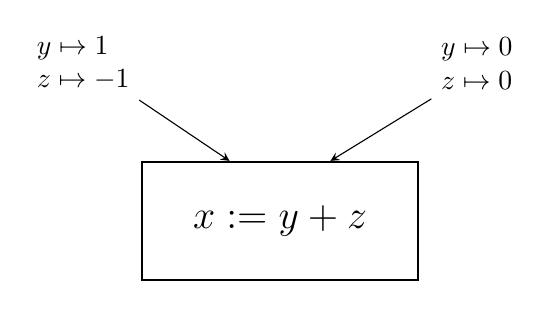
\begin{tikzpicture}
        % Nodo sinistro (Stato s0)
        \node[align=left] (left_state) at (-2.5, 2) {
            $y \mapsto 1$ \\
            $z \mapsto -1$
        };

        % Nodo destro (Stato s1)
        \node[align=left] (right_state) at (2.5, 2) {
            $y \mapsto 0$ \\
            $z \mapsto 0$
        };

        % Box centrale (Istruzione)
        \node[draw, thick, minimum width=3.5cm, minimum height=1.5cm] (instruction) at (0, 0) {
            \Large $x := y + z$
        };

        % Frecce
        \draw[->, >=stealth] (left_state.south east) -- (instruction.130);
        \draw[->, >=stealth] (right_state.south west) -- (instruction.50);
    \end{tikzpicture}
\end{center}

Dal CFG sopra è possibile costruire due insiemi di stati:
\begin{itemize}
    \item Stato $s_0$ (nodo sinistro): $ \{ y \mapsto 1, z \mapsto -1 \} $
    \item Stato $s_1$ (nodo destro): $ \{ y \mapsto 0, z \mapsto 0 \} $
\end{itemize}

La funzione di trasferimeno al join point (l'istruzione $x := y + z$) calcola il
nuovo stato:
\[
f(s_{in}) = f(s_0 \sqcup s_1)
\]
dove $\sqcup$ è l'operatore di join del reticolo CP.

Per verificare se la constant propagation è distributiva, è necessario calcolare
$f(s_0 \sqcup s_1)$ e confrontarlo con $f(s_0) \sqcup f(s_1)$.:
 

Prima di eseguire l'istruzione, l'analisi unisce le informazioni provenienti
dai due rami:
\begin{itemize}
    \item Per $y$: $1 \sqcup 0 = \top$.
    \item Per $z$: $-1 \sqcup 0 = \top$.
\end{itemize}
Quindi lo stato unito è $s_{join} = [ y \mapsto \top, z \mapsto \top ]$.


Successivamente l'analisi valuta $x := y + z$ usando lo stato $s_{join}$:
\[ x := \top + \top \implies x \mapsto \top \]
Quindi $f(s_0 \sqcup s_1) = [ x \mapsto \top, y \mapsto \top, z \mapsto \top ]$,
portando al risultato che $x$ non è costante.

\medskip

Tuttavia, se l'analisi fosse distributiva si dovrebbe ottenere lo stesso
risultato unendo i risultati delle singole esecuzioni ($f(s_0) \sqcup f(s_1)$):

\begin{itemize}
    \item Nel ramo sinistro ($s_0$): $x := 1 + (-1) = 0$.
    \item Nel ramo destro ($s_1$): $x := 0 + 0 = 0$.
    \item Unione dei risultati: $0 \sqcup 0 = 0$.
\end{itemize}

Poiché il risultato reale dell'analisi ($\top$) è diverso e meno preciso del risultato ideale ($0$):
\[ f(s_0 \sqcup s_1) \neq f(s_0) \sqcup f(s_1) \]
\[ \top \neq 0 \]
si dimostra che la propagazione delle costanti non è un'analisi distributiva.

\end{nota}
\section{Introduzione a LiSA e architettura di un analizzatore statico}

\subsection{Panoramica di un analizzatore statico}

Un analizzatore statico è composto da diversi componenti modulari che
interagiscono per trasformare il codice sorgente in un risultato di analisi
(es. warning o garanzie di correttezza).


\begin{definizione}{Componenti Principali}{static_analyzer_components}
Il flusso di un analizzatore statico può essere riassunto nei seguenti
passaggi logici:
\begin{itemize}
    \item \textbf{Programma}: Il codice sorgente in input.
    \item \textbf{IR}: Il programma viene tradotto in una rappresentazione
    interna che è più facile da analizzare.
    \item \textbf{Engine di analisi}: Il cuore dell'analizzatore che gestisce
    l'algoritmo di punto fisso, la risoluzione delle chiamate e la gestione
    della memoria.
    \item \textbf{Dominio}: L'astrazione dei dati su cui lavora l'algoritmo
    (es. propagazione delle costanti, intervalli).
\end{itemize}

\begin{figure}[H]
  \centering
  
\includegraphics[width=0.6\textwidth]{images/th_05/01.png}
  \caption{L'immagine illustra i componenti principali di un analizzatore
  statico.}
  \label{fig:th_05_01}
\end{figure}
\end{definizione}

\begin{nota}{Modularità}{modularity_lisa}
Una domanda fondamentale nella progettazione di un analizzatore è:
``Come cambiare l'analisi o il linguaggio senza riscrivere tutto?''.
La risposta risiede nell'indipendenza dei componenti:
\begin{itemize}
    \item I componenti dell'analisi devono essere indipendenti l'uno
    dall'altro.
    \item I componenti dell'analisi e la IR non devono essere modellati su
    uno specifico linguaggio sorgente.
\end{itemize}
Questo permette, ad esempio, di cambiare il dominio astratto (da costanti a
intervalli) senza modificare l'algoritmo di visita.

\begin{figure}[H]
  \centering
  \includegraphics[width=0.6\textwidth]{images/th_05/02.png}
  \caption{L'immagine illustra una possibile scomposizione modulare di un
  analizzatore statico.}
  \label{fig:th_05_02}
\end{figure}

\end{nota}

\subsection{LiSA}

LiSA (Library for Static Analysis) è una libreria open-source scritta in Java
per la realizzazione di analizzatori statici basati su interpretazione astratta.

\subsubsection{Overview}
In LiSA, il codice sorgente viene tradotto da un front-end specifico per i
linguaggio (es. per Java o IMP) in una collezione di control flow graph.

\begin{figure}[H]
  \centering
  \includegraphics[width=0.8\textwidth]{images/th_05/03.png}
  \caption{L'immagine illustra il flusso di analisi in LiSA.}
  \label{fig:th_05_03}
\end{figure}


\begin{definizione}{Struttura di un CFG in LiSA}{lisa_cfg}

Un CFG in LiSA è costituito da:
\begin{itemize}
    \item Un insieme di nodi, che rappresentano gli statement del programma.
    \item Un insieme di archi che collegano i nodi.
\end{itemize}

Gli archi possono essere di tre tipi:
\begin{itemize}
    \item \textbf{Sequential edge:} Flusso di esecuzione sequenziale standard.
    \item \textbf{True edge:} Preso quando la condizione del nodo sorgente è
    valutata come vera (assumed to hold).
    \item \textbf{False edge:} Preso quando la condizione del nodo sorgente è
    valutata come falsa (assumed not to hold).
\end{itemize}


\begin{figure}[H]
  \centering
  \includegraphics[width=0.8\textwidth]{images/th_05/04.png}
  \caption{L'immagine illustra la struttura di un CFG in LiSA.}
  \label{fig:th_05_04}
\end{figure}

\end{definizione}


L'utilizzo dei CFG permette di astrarre dalla sintassi specifica del controllo
di flusso del linguaggio originale (es. cicli while, for, if) e definire
algoritmi di punto fisso direttamente sul grafo.

\subsection{Sintassi vs Semantica}

Un concetto chiave in LiSA è la distinzione tra lo statement sintattico
(il nodo del CFG) e il suo significato semantico.

\begin{nota}{Il problema della sintassi}{syntax_problem}
Uno statement potrebbe essere complesso e avere diverse rappresentazioni
sintattiche equivalenti oppure diverse operazioni sintattiche
possono avere la stessa semantica. Ad esempio, in Java, \texttt{``a'' + ``b''}
e \texttt{``a''.concat (``b'')} eseguono entrambi una concatenazione di
stringhe.

Un dominio astratto non dovrebbe preoccuparsi di come l'operazione è
scritta sintatticamente.
\end{nota}

Per risolvere questo problema, LiSA utilizza un linguaggio interno di
\textbf{symbolic expressions}. Così facendo:
\begin{itemize}
    \item I domini lavorano su espressioni simboliche, non sugli
    statement grezzi.
    \item Ogni espressione simbolica rappresenta un'operazione semantica
    ``atomica'' (es. somma aritmetica, concatenazione stringhe).
    \item Durante il calcolo del punto fisso, il metodo
    \texttt{Statement.semantics ()} riscrive lo statement in una o più
    espressioni simboliche da passare al dominio.
\end{itemize}

\begin{esempio}{Rewriting semantico}{semantic_rewriting}
Consideriamo un operatore \texttt{Plus} generico. La sua semantica potrebbe
essere definita come:
\begin{itemize}
    \item Se gli operandi sono stringhe $\rightarrow$ ritorna una
    \texttt{StringConcat}.
    \item Altrimenti $\rightarrow$ ritorna una \texttt{ArithmSum}.
\end{itemize}
Il dominio astratto implementerà poi la logica specifica per
\texttt{StringConcat} o \texttt{ArithmSum}.

\begin{figure}[H]
  \centering
  \includegraphics[width=0.4\textwidth]{images/th_05/05.png}
  \caption{L'immagine illustra lo pseudocodice dell'operatore \texttt{Plus}.}
  \label{fig:th_05_05}
\end{figure}

\end{esempio}

\subsection{Implementazione dell'analisi dataflow}

LiSA fornisce un'architettura specifica per implementare le analisi dataflow
(Vedi \ref{subsec:dataflow_analysis}).

\begin{definizione}{Dataflow in LiSA}{lisa_dataflow}
Le analisi dataflow in LiSA sfruttano l'algoritmo di punto fisso generico
basato su worklist.

\begin{figure}[H]
  \centering
  \includegraphics[width=0.6\textwidth]{images/th_05/06.png}
    \caption{L'immagine illustra l'algoritmo di punto fisso generico basato
    su worklist per l'analisi dataflow forward, evidenziando in rosso i
    componenti che variano in base alla semantica dell'analisi (May vs Must)
    e che necessitano di essere modularizzati.}
  \label{fig:th_05_06}
\end{figure}

L'implementazione è divisa in due classi principali per separare la gestione
del reticolo dalla logica di trasferimento:

\begin{itemize}
    \item \textbf{DataflowDomain}: Gestisce la logica generale del dominio,
    inclusa la valutazione delle espressioni e degli assegnamenti.
    Esistono due specializzazioni principali basate sul tipo di join:
    \begin{itemize}
        \item \textbf{PossibleForwardDataflowDomain} che implementa un'analisi
        \textit{May} (possibile). L'operazione di \texttt{lub} (join) è
        l'unione degli insiemi.
        \item \textbf{DefiniteForwardDataflowDomain} che implementa un'analisi
        \textit{Must} (definita). L'operazione di \texttt{lub} (join) è
        l'intersezione degli insiemi.
    \end{itemize}
    
    \item \textbf{DataflowElement}: Rappresenta il singolo elemento tracciato
    dal dominio. Questa classe definisce le operazioni specifiche di
    \textbf{gen} e \textbf{kill}.
\end{itemize}

\begin{figure}[H]
  \centering
  \includegraphics[width=0.8\textwidth]{images/th_05/07.png}
  \caption{L'immagine illustra lo schema delle classi per l'analisi dataflow
  in LiSA.}
  \label{fig:th_05_07}
\end{figure}

\end{definizione}

\begin{nota}{Tipi di analisi supportate}{lisa_analysis_types}
Attualmente, LiSA supporta esclusivamente analisi di tipo \textbf{forward}.
Per quanto riguarda la semantica dell'analisi, sono supportate sia le
analisi \textit{May} (possibile) che \textit{Must} (definita).
\end{nota}

\end{document}